\section{Diffusion Tensor Imaging}
Diffusion is a process that involves the movement of molecules via thermally driven random motions, or namely Brownian motion (see Figure \ref{fig:diffusion}). Generally, factors such as molecular weight, viscosity, and temperature are the common solution properties influencing diffusion. However, in biological tissues, the cellular organization of the tissue influences the mobility of diffusing molecules by acting as obstacles within our organs. In certain cases, this means that the distance traveled by a diffusing molecules in one direction will not be the same as some other directions. As a comparison, in a solution with no barriers to diffusion, diffusion is isotropic or the same in all directions (See Figure \ref{fig:diffusion}, middle). On the other hand, if diffusion is hindered by some particularly oriented barriers, then it is termed anisotropic diffusion (Figure \ref{fig:diffusion}, right). In the anisotropic scenario, the structural organization of the barriers can be identified simply by the diffusion patterns and the degree of anisotropy is directly related to the geometry of the barriers. 

\begin{figure}[htbp]
	\centering
	\includegraphics[width=\textwidth]{../figures/chapter2/motion_diffusion.png}
	\caption{Illustrations of diffusion}
	\caption*{Left: Diffusion process illustrated by simulated Brownian motion where four particles, indicated by different colors, all begin at the same origin of $(0,0)$ yet end up with different random paths. In biological tissues, diffusion path of water molecules will be influenced by cellular microstructures. Middle: cartoon illustrating diffusion with similar molecular displacement in all directions (isotropic). Right: cartoon illustrating greater diffusion in one direction over others (anisotropic).}
	\label{fig:diffusion}
\end{figure}

Diffusion weighted imaging(DWI) takes advantage of the phenomenon that water diffusion is highly anisotropic in tissues of the nervous system. In magnetic resonance imaging techniques, diffusion is often measured by an  "apparent diffusion coefficient" (ADC). Which is not a \emph{true} measure of the intrinsic diffusion, but instead a metric dependent on the interaction of the molecule (water in most biological usages) with the cellular structures over a given amount of diffusion time. In contrast to DWI, diffusion tensor imaging (DTI) computes a diffusion tensor that's a 3-by-3 matrix instead of one numerical value. This 3D tensor allows estimates of water mobility in all directions for a given voxel, enabling quantification of anisotropic diffusion. The methodology to combine diffusion metrics with magnetic resonance pulses was introduced by Stejskal and Tanner in 1960 \cite{stejskal_spin_1965}, and eventually adapted to clinical routines by Le Bihan and colleagues in 1980 \cite{le_bihan_mr_1986}. The key idea in this adaptation is that stationary water spin signal will be the same in response to two magnetic pulses of opposite polarities, but  moving water will return spin signals in a different position, giving off a weaker signal. The difference in signal attenuation is proportional to the water motion. Modern DTI acquisition routines reduce scan time by sending a series of oscillation gradient reversals instead of a train of $180^{\circ}$ pulses. Water movement is sampled in all directions covered by the diffusion sensitive gradients, providing quantification of diffusion in $x,y,z$ directions of a 3D brain volume. 

% Insert DWI figure illustrating directionality
\begin{figure}[htbp]
	\centering
	\includegraphics[scale=0.8]{../figures/chapter2/fod.png}
	\caption{Axial view of human brain's fiber orientation distribution.}
	\caption*{Tri-dimensional representation of water diffusion along white-matter fibers with color coded $x \textrm{ (red)},y\textrm{ (green)},z\textrm{ (blue)}$ axes representing main diffusion direction. Spherical models provide information about the degree of anisotropy, with longer poles representing directed diffusion and smaller spheres representing isotropic diffusion. Zoomed in region showing anisotropic diffusion along the corpus callosum.}
	\label{fig:fod}
\end{figure}

% Summarize dMRI, last few points, transition to usages with citations, and finally transition to why and what we do here.
The concept of diffusion coefficient is only briefly covered here, as there has been much more sophisticated methods of quantifying anisotropic diffusion \cite{basser_estimation_1994, basser_mr_1994,pierpaoli_toward_1996,ulug_orientation-independent_1999}. However, the simple ADC framework provides an intuitive feel for diffusion tensors and has led to many valuable findings. Early observations of water diffusion in human brains in vivo focused on areas of large diffusion variation. Measurements showing a range of diffusion constants in white-matter fibers with different gradients revealed myelinated sheaths, microfilaments, and axonala membranes can act as barriers to water molecules traveling along the length of axons \cite{thomsen_vivo_1987}. On the other hand, gray matter does not exhibit anisotropic diffusion due to the lack of long oriented fiber structures \cite{chenevert_anisotropic_1990, chien_mr_1990}.  Subsequently, studies showing anisotropic water diffusion in animal brains and spinal cords \cite{moseley_diffusion-weighted_1990,king_diffusion-weighted_1991,howe_magnetic_1992} in addition to human cranial nerves \cite{hajnal_mr_1991,moseley_anisotropy_1991} proved the usefulness of diffusion weighted MRI. Eventually, DTI was adapted for measuring brain maturation \cite{sakuma_adult_1991,rutherford_mr_1991} as well as non-invasive fiber orientation \cite{douek_mr_1991}. 

\subsection{Diffusion MRI Drawbacks}
While diffusion tensors became even more widely adapted with modern neuroscience studies acquiring multiple modalities of brain images at the same time, improving the signal to noise ratio (SNR) of DWI contrasts and accuracy of tensors have also shifted into focus. Despite its clinical usages for both brain \cite{moseley_diffusion-weighted_1990,warach_acute_1995} and body \cite{kiselev_fundamentals_2017,koh_diffusion-weighted_2007}, a low signal to noise ratio and artifact contamination are usual sources of low confidence in diffusion measurements. Specifically, long scan echo times (60-120 ms) and strong diffusion gradient pulses limits precision, and subsequently the accuracy of diffusion estimations after acquisition \cite{aja-fernandez_noise_2008,veraart_constrained_2011}. Aside from post hoc digital processing, improved SNR can be achieved by lengthening scan time or lowering spatial resolution. Longer scan times for each gradient direction only increases precision slowly, while echo times imposed by hardware  and acquisition protocol prevents changes in scan time. Additionally, loss in anatomical detail and smoothing effects contradicts the goal of improving SNR by lowering spatial resolution. 

Unlike hardware imposed SNR deficits, diffusion MRI in humans suffers from additional artifacts from a variety of sources. While all MR acquisitions experience degrees of motion artifacts, diffusion MRI is exceedingly sensitive to motion. During  the strong gradient pulses, any head motion or small tissue movement such as pulsating flow amplifies the detected shifts in molecules. If all spin shifts detected in all voxels experience the same motion displacement, there is minimal loss in signal coherence and effects on ADC measurements. However, problematic artifacts occur when voxels in different slices of MR acquisition experience different degrees of motion during a single MR pulse sequence. In addition, macroscopic head motion will not be identical replicas of itself every time, and an accumulation of shifts over time during a sequence of pulses will lead to large signal variations across the image\cite{le_bihan_artifacts_2006}. Another artifact arising from repeated gradient pulse switches is eddy currents, where conducting surfaces in the MRI machinery induct currents in response to the on-off switching of magnetic pulses, which results in erroneously persisting gradients in addition to the main gradient \cite{andersson_model-based_2002,andersson_integrated_2016}. As mentioned before, low spatial sampling resolution to shorten scan time is common in diffusion MRI acquisition protocol, the effect of this shortcoming is exacerbated when high-contrast boundaries are poorly sampled, leading to Gibbs ringing artifacts \cite{veraart_gibbs_2016,wheeler_2021,tournier_diffusion_2011}. Such boundary artifacts have been identified to cause inaccuracies such as erroneous negative diffusivity and kurtosis values (kurtosis map black voxels) \cite{veraart_gibbs_2016,kellner_gibbs-ringing_2016,perrone_effect_2015}. Lastly, spatial signal bias caused by radio frequency pulse inhomogeneity which also requies correction \cite{bernstein_imaging_2006,belaroussi_intensity_2006}. 

\section{DESIGNER Pipeline}
Improving diffusion tensor estimates via spatial smoothing \cite{tabesh_estimation_2011} or averaging \cite{cui_panda_2013} are considered brute force techniques that do not specifically target a type of contamination such as Gibbs ringing or thermal noise. To amend the noise and artifact issues mentioned above, Ades-Aron and colleagues proposed the DESIGNER pipeline, which stands for "Diffusion parameter EStImation with Gibbs and NoisE removal" \cite{ades-aron_evaluation_2018}. This preprocessing pipeline was shown to increase diffusion estimation precision by a factor of ~2 compared to aforementioned pipelines while preserving spatial resolution. Since then, specific proposed procedures in DESIGNER has been adapted into the open source software \emph{mrtrix3} \cite{tournier_mrtrix3_2019}. 

\emph{Mrtrix3} provides a large collection of functionality for diffusion MRI focused processing and analysis. Similar to older pre-existing tools such as Freesurfer \cite{Fischl2012}, SPM \cite{penny_statistical_2006}, and FSL \cite{Jenkinson2012}, the suite of neuroimaging tool provide standalone modules but do not have any pre-established workflows, capabilities for parallel processing across subject data, or a standardized input \& output data framework. Although the DESIGNER pipeline is available as an open source Python project, the simple scripts does not comprehensively cover end-to-end diffusion MRI processing, and is not easily scalable to large datasets. Here, we will summarize the problems and preprocessing procedures recommended by DESIGNER, introduce our contributions to automating diffusion MRI processing, and showcase collaborative efforts on accelerating diffusion derived tractography computations.

\subsection{MP-PCA}
The pre-requisite step before targeted artifact removal is to denoise, as corrupted spatially varying MRI data can propagate through preprocessing procedures and lower the accuracy of the final diffusion quantification \cite{vizioli_lowering_2021}. 

\subsection{Pipetography Pipeline}

\section{Tractography}
Tractography based on diffusion-weighted MRI provides non-invasive in vivo estimates of trajectories of long-range brain connections. These estimates are important in research that measures individual differences in brain connections and in clinical use-cases. But the computational demands of tractography present a barrier to progress. Here, we present a GPU-based tractography implementation that accelerates tractography algorithms implemented as part of the Diffusion Imaging in Python (DIPY) project. This implementation speeds up tractography by at least a factor of ~200X, providing tractographies that closely match CPU-based solutions. These speedups enable applications of tractography in clinical data, and in very large datasets.

\subsection{GPU-accelerated Diffusion MRI Tractography in DIPY}
DIPY (Diffusion Imaging in Python; \url{https://dipy.org}) is an open-source software library that implements many methods in computational neuroanatomy \cite{garyfallidis_dipy_2014}. Relying on the DIPY implementation of residual bootstrap tractography \cite{berman_probabilistic_2008}, we implemented a multi-GPU parallelizable version constructed on NVIDIA’s CUDA application programming interface (API).  The API of the GPU version is compatible with the one implemented in DIPY, enabling direct comparisons and interoperability. A docker container of the software makes the installation and use of the software straightforward. The software is available at \url{https://github.com/dipy/GPUStreamlines}. Experiments to profile the performance of the algorithm were conducted using an AWS $p3.16\textrm{xlarge}$ instance with 8 NVIDIA Tesla V100 Graphical Processing Units and 488 GB RAM. For comparison, CPU code was run on an AWS $x1e.4\textrm{xlarge}$ with 488 GB RAM. We used two datasets, the first is a HARDI acquisition with 2x2x2 mm3 isotropic voxels, 150 b=1,000 s/mm2 volumes and 10 b0 volumes previously described in \cite{rokem_evaluating_2015}. The other dataset was a Super-Resolution Hybrid Diffusion Imaging  (HYDI) dataset \cite{Garyfallidis2019}, with an effective resolution of 0.625 mm3 isotropic voxels, b=500, 800, 1600, 2600 s/mm2, in 134 diffusion directions, and 8 b0 volumes, also previously described in \cite{elsaid_super-resolution_2019}. In both cases, 27 seeds were placed in each voxel in the white matter to initialize tracking.

\subsection{Results} 
In the HARDI dataset, with the seeding approach used
here, approximately 2.1M streamlines were generated. Using the CPU-based
residual bootstrap tracking algorithm took approximately 13 hours. The
GPU-accelerated implementation provides approximately 200-fold speedup
with a single GPU, and up to 671-fold speedup with 8 GPUs run in
parallel (Figure \ref{fig:gpu_speedup}). In the HYDI dataset, the seeding approach used generated 150M streamlines (497GB). Tracking in this case with 8 GPU
completed in just under 2 hours. A subset of the HYDI streamlines are
shown in Figure \ref{fig:gpu_streamlines}.

\begin{figure}[htbp]
    \centering
    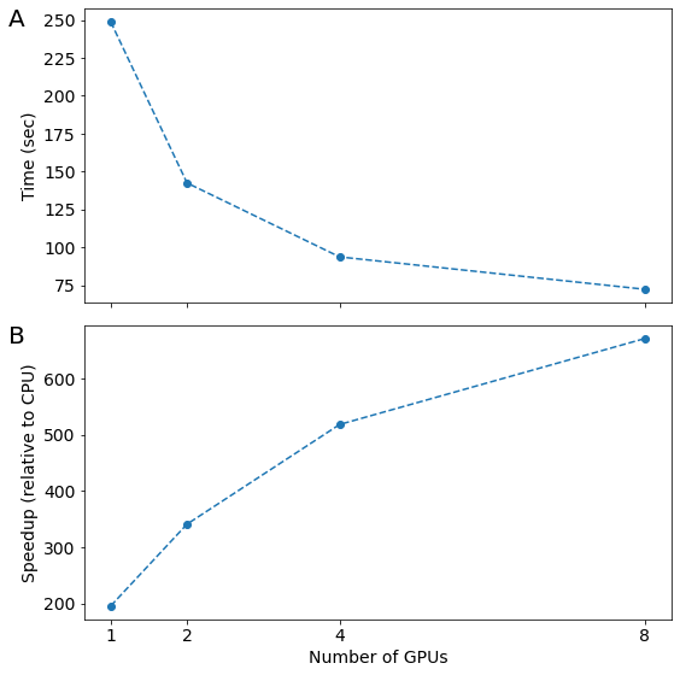
\includegraphics[width=\textwidth]{../figures/chapter2/speedup.png}
    \caption{GPU streamline generation speedup compared to CPU}
    \caption*{For the same task (HARDI data, 27 seeds per WM voxel) tractography duration decreases with the number of GPUs available. Speedup relative to CPU ranges from approximately 200-fold, with one GPU to almost 700-fold with 8 GPUs.}
    \label{fig:gpu_speedup}
\end{figure}

\begin{figure}[htbp]
	\centering
	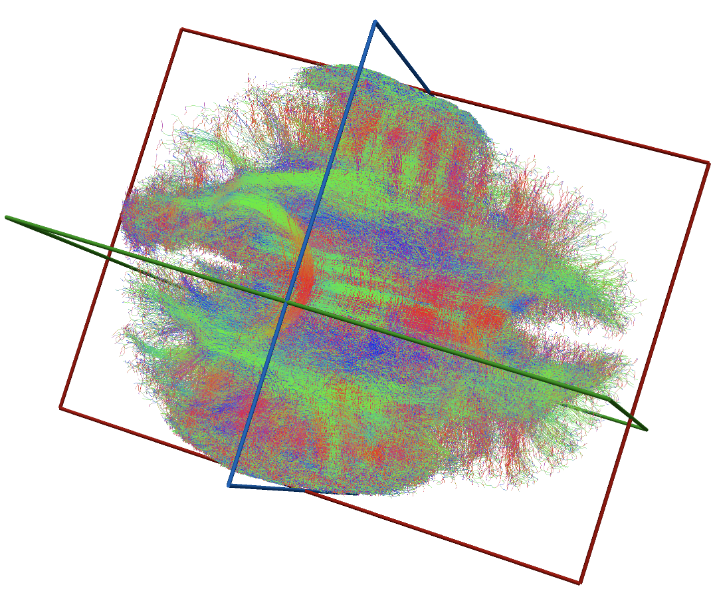
\includegraphics[width=\textwidth]{../figures/chapter2/streamlines.png}
	\caption{Visualization of GPU generated streamlines.}
	\caption*{GPU-accelerated tractography of high-resolution data, acquired at 0.625 mm3  effective resolution. This is a small subset sampled randomly for visualization purposes: approximately 8M streamlines of the 150M streamlines tracked.}
	\label{fig:gpu_streamlines}
\end{figure}

\subsection{Discussion and Conclusion} 
A GPU-based implementation of residual bootstrap tractography provides orders of magnitude speedup, relative to the CPU-based version, while providing solutions that match CPU-based solutions very closely. This was demonstrated in standard and high-resolution measurements. Thus, this GPU-based implementation allows
researchers to both (1) save time and money solving existing problem
sizes and (2) solve new problems that are computationally intractable on
CPU-only resources. Open-source software is provided, as well as a
docker container that encapsulates the software, together with all of
its dependencies available at
\url{docker.pkg.github.com/dipy/gpustreamlines/gpustreamlines}.
